\subsection{Health and Safety}\label{subsec:healthnsafety}

Since we are working on a pure software project,
we do not interact with any dangerous tools or hardware.
The most fearsome tools for us are actually our office peripherals.
We need to be conscious of the ergonomics of our work environment.


% TODO: add ref, https://www.ccohs.ca/oshanswers/ergonomics/office/monitor_positioning.html
Monitor placement is important because it affects eye strain, and postural strain (neck and shoulders).
It is recommended to keep the monitor approximately forty to seventy cm away from the eyes.
For a quick reference, this is roughly an arm's length away, but it depends on the person.
The monitor height is important as well.
In general, research has found that eyes naturally have a downward cast. % REF.
In fact, they strain more looking above, than looking down.
In practice, guidelines recommend keeping the top of the monitor at eye level, or slightly below.
In general, these are just guidelines to get a good starting point.
It may be worth experimenting depending on the individual's body and what feels best.
A visual summary of these recommendations is given by the Canadian Centre for Occupational Health and Safety (CCOHS) in Figure~\ref{fig:monitor-pos}. % TODO Ref here
\begin{figure}[h]
    \centering
    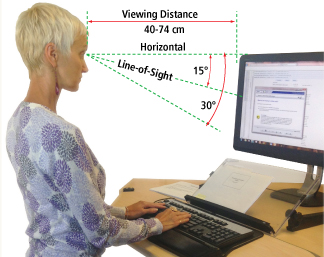
\includegraphics[width=0.5\textwidth]{monitorposition1}
    \caption{The recommended monitor position guidelines from CCOHS.}
    \label{fig:monitor-pos}
\end{figure}

When working for excessively long periods of time without breaks,
it is possible to get repetitive strain injuries (RSI).
It can be from clicking the mouse too much or typing a lot on the keyboard.
Certain mice and keyboards are more ergonomic and help reduce these strains.
They usually have aggressive curves forcing your body to adopt more ergonomic poses.
Office chairs are also an important part of ergonomics, providing proper support while sitting at a desk.

However, even with the best ergonomics setups, the most important is to take frequent breaks from the computer.
Getting up, then walking is good to reduce eye strain, as well as reducing the chances of getting an RSI.
To do this reliably, it is best to set timers and respect them.
Otherwise, there is a risk of getting too absorbed in the work.
After 8 hours of work without breaks writing a report, hands start aching and your body will be the one demanding a break.

% subsection  (end)

\subsection{Engineering Professionalism}\label{subsec:engineering-professionalism}
In ECOR4995, we learned that safety was paramount.

Our first step in addressing this was to analyze the security concerns of our tool.
We do not believe there to be any security vulnerabilities.
This is because it is completely local to the machine, with no internet connection.
We do not believe someone using our tool can harm someone other than themselves by intentionally misusing it.
The only concern would be if an individual delivers falsifies the outputs to provide to someone else.
However, we provide no guarantee for this.
We create text files that can be spoofed without our tool even existing, we decided this concern to be out of scope.

The next question is are there safety concerns, were users can cause harm unintentionally?
We believe there is a way to do so, if our outputs provide false information to a designer.
If the analyzed system is safety critical this can become a safety concern.
The analysis done with our faulty outputs would then compromise the analysis of the safety critical system.
To guard against this, accuracy of our outputs became a critical requirement in our user requirements (see section~\ref{subsubsec:user-reqs}).
We even have a second requirement preferring failure over false positive outputs.

We also made sure to properly licence our program, since we learned that intellectual property was pretty important.

\subsection{Project Management}\label{subsec:project-management}
We started the project by defining some processes for baseline communication and work hours.
That strategy did not work well because we still faced long periods of time without any work or communication.
We had weekly meetings at first, but we wasted time because we had multiple weeks with no work.

The crux of our recovery from this disastrous start came from a pivot towards asynchronous project management with \textbf{GitHub Issues}.
We will look at their purpose in more detail in section~\ref{subsubsec:proj-mngmnt}.
In summary, they were used to formulate task units at a lower level than our requirements.
We could also self-assign the tasks we wanted to do to show to everyone we started work on it.
This is to have a person to contact for status updates, or permission to collaborate on it and avoid duplicating work.

In practice, we stopped doing the assignments because only one person was working for a long period of time.
During the last week before the fair, the team became slightly more active.
Project Management went back to synchronous meetings with dedicated task assignments,
and frequent check-ups to ensure no one was blocked for too long.

We also defined timelines, but they were not respected either.
They only served as a reminder that we were permanently behind schedule, even when we revised our timeline later.
When we switched to Issues, we ended up somewhat ignoring timelines.
We were already working as much as possible until we got blocked, typically due to some lack of understanding of C2KA\@.

Having said that, we still had a clear roadmap of features to follow, and a target date for a first prototype (the fair).
When we were planning tasks, we asked ourselves the feasibility of completion.
This was done in an adhoc manner, based on our knowledge of the current system, and the work left to do.
As we went, we also made sure to mark out of scope features whenever possible (with a rationale) to increase feasibility.

\subsection{Degree Suitability}\label{subsec:deg-suit}

\subsubsection{Alexandre Marques}
This project was suitable to my degree because it touches on many concepts I've learned in class.
It is an engineering project, and it is a software project so it is natural that it fits my Software Engineering degree.
More specifically:
\begin{itemize}
    \item I've applied Project Management techniques from SYSC4106 to increase the chances of completing the project
    \item I've applied Object-Oriented design patterns from SYSC3110 to improve program maintainability and capabilities
    \item I've applied Verification \& Validation concepts from SYSC4101 to increase quality
    \item I've applied CI/CD concepts from SYSC4806 to streamline our development process
    \item I've applied program architecture pattern knowledge from SYSC4120 to select and implement the Pipe and Filter pattern as the best architecture for our goals.
    \item I've applied my knowledge of programming languages from SYSC3101 to select the best language for our needs.
    \item I've applied requirement engineering techniques from SYSC3120 to write a set of functional and non-functional requirements for our program.
    \item I've applied induction rules from COMP2804, COM1805 to implement the recursive logic needed to convert C2KA diagrams (technically learned in SYSC2100 but discrete math taught me recursion much better).
    \item I've applied my Operating System knowledge from SYSC4001 to work on multiple OS hosts and make the IIAT work.
    \item I've applied my knowledge of formal methods from SYSC4111 to identify the importance of formal languages and understand C2KA better.
    \item I've applied my knowledge of modelling from SYSC5805 and SYSC5104 to understand the importance of models in the engineering process.
    \item I've applied my experience in writing technical reports from an academic research internship I've done before the degree,
    combined with the LaTeX skills I've learned during the degree submitting assignments in various classes.
    Although the internship was not part of my degree, it was valuable relevant experience in this domain.
    I was only offered the opportunity because I aimed to do something related to software before even starting the degree.
    \item I've omitted some pre-requisite classes which were not directly relevant,
    but they also contributed to giving me the capabilities to complete this project.
    \item I don't remember when we learned UML and state diagrams.
    It feels like we see them all the time in different classes.
    That was important pre-requisite knowledge too.
\end{itemize}


\subsubsection{Michael Rochefort}\label{subsubsec:mike-deg}

This capstone project integrates and applies a broad range of skills and knowledge from the Software Engineering degree, demonstrating its suitability as a culminating project for the program. At its core, the project required engineering a complex software system from conception to verification, which aligns perfectly with Software Engineering principles. We began with requirements analysis (identifying what the tool needs to do and under what constraints), a process learned in our Requirements Engineering courses. We then moved to software design, selecting an architecture (pipe-and-filter) and design patterns appropriate for the problem. This reflects knowledge from software architecture and design courses, where evaluating and applying architectural styles is a key learning outcome. The implementation involved writing a substantial amount of code in an organized manner, applying best practices for coding and documentation that we developed throughout my degree. Notably, the project’s focus on converting UML models to formal specifications bridged theory and practice: we utilized UML modelling techniques taught in modelling and software design classes, and we engaged with formal methods by generating specifications.

The project also demanded proficient use of software engineering tools and practices. For instance, we used version control (Git/GitHub) extensively – a skill emphasized in our software engineering labs – to collaborate and manage our codebase. We practiced issue tracking and agile-like iteration, echoing project management coursework, to keep the team organized and responsive to changes. The testing strategy we used is a direct application of software testing principles learned in class; we wrote unit tests, integration tests, and system tests much as we would in an industrial setting, reinforcing our understanding of testing frameworks and the importance of test coverage.

Lastly, this project involved teamwork and communication, soft skills that are integral to the Software Engineering program. We had to collaborate effectively, divide tasks, conduct code reviews, and integrate our work, which mirrors the team projects and assignments throughout my degree. The production of a comprehensive technical report and documentation tested my technical communication skills, another key component of the program’s outcomes.


\subsubsection{Ahmed Babar}\label{subsubsec:ahmed-deg}
The Goal of this project is to streamline and reduce error by creating an automated input for an existing error analysis tool. This project is suitable for the software development degree program as it demonstrates Object oriented programming picked up from courses like 3303 and 2006 where multithreading is used to improve efficiency and 2006 where coupling and techniques were used to create object oriented project just like this one. Another example of use of knowledge from previous course related to this degree include 4001 software validation and 4120 and 3120.

\subsection{Individual Project Contributions}\label{subsec:individual-project-contributions}
\subsubsection{Alexandre Marques}
% TODO: A lot more!!!
\begin{itemize}
    \item TODO: I did everything not included by them, their sections are comprehensive.
    It will take a while to write mine, taking a break.
    \item Fixed draft Manufacturing Cell diagrams in Papyrus to be accurate and testable according to our input specifications
    \item Analyzed state diagrams and drew conclusions on elements of interest for our C2KA transformations.
    Later, revisited this idea by trying to formalize it through C2KA base representations.
    \item Researched C2KA to develop a deep understanding of possible transformations,
    and attempted to form a solid testing basis by creating C2KA Base Representation diagrams % TODO ref paper here
    \item Documented rules and possible mappings of C2KA in an internal wiki, using the Base Representations for reference. % TODO Add wiki as appendix?
    \item Code reviewed all the pull requests in the repository, providing meaningful feedback to improve code quality.
    \item Refactored integration tests and streamlined testing by creating reusable pipelines.
    \item Refactored tests to import test paths, and the diff tool as re-usable utilities.
\end{itemize}

\subsubsection{Michael Rochefort}
\begin{itemize}
    \item Helped figure out comment parsing in diagrams (dropped feature).
We did use this knowledge later to understand how to configure the parser for our needs.
    \item Did research on Dijkstra's Guarded Command Language (GCL), and the transformations between its syntax and the IIAT.
    Documented these findings in an internal wiki.
    \item Drew the C2KA base model diagram in Papyrus related to concrete behavior containing a conditional statement written in GCL.
    \item Wrote an integration test case for StateDiagramLinker using the C2KA base model with the GCL concrete behavior.
    \item Created the accuracy validation diff tool which matches agent specification irrespective of order, with the same semantic meaning.
\end{itemize}

\subsubsection{Ahmed Babar}
\begin{itemize}
    \item Created draft Manufacturing Cell diagrams in Papyrus for all agents (with many errors)
    \item Did research on State Diagrams, with no clear goal or conclusion.
    Documented a lot of irrelevant information making it unclear how to use state diagrams for C2KA derivations.
    \item Started adding integration test cases to StateDiagramLinker according to a template,
    but could not complete them to an adequate level of quality in time.
    \item Started (but failed to complete) creation of Wastewater system diagram inputs in Papyrus for a second system test.
\end{itemize}

\subsection{Individual Final Report Contributions}\label{subsec:individual-final-report-contributions}
Ahmed wrote section~\ref{subsubsec:ahmed-deg}
Micheal wrote section~\ref{subsubsec:mike-deg}.
However, the work to port both sections to LaTeX from the draft report was done by Alexandre Marques.

Everything else was written by Alexandre Marques.
This includes all formatting, figure creation, setting up the LaTeX environment, etc.
Figure creation does include creating new diagrams, running the IIAT tool,
figuring out why it was breaking, etc.
All the work relating to formally defining requirements and tracing their fulfillment was done as a part of this report.

All sections from the draft unless otherwise mentioned above were re-written from scratch by Alexandre Marques to incorporate the feedback.
As a disclaimer, this includes project contributions in section~\ref{subsec:individual-project-contributions}
which were edited from the draft report for accuracy by Alexandre Marques.